\problemname{Tycho}

\illustration{.4}{img/MarsPerseveranceRover.jpg}{}

\noindent
Rum\-udforsknings\-køretøjet \emph{Tycho VIII} skal tilbage til hjemmebasen efter at have indsamlet mineralprøver.
Tycho bevæger sig i en lige linje fra position~$0$ til hjemmebasen ved position~$b$.
Når den bevæger sig, flytter den sig med en langsom, men stabil hastighed på $1$~enhed pr.\ sekund.
Hvert sekund tager Tycho $1$~enhed miljøskade fra de barske forhold på planeten.

Situationen forværres desuden af strålingen fra en nærliggende pulsar, der tilføjer $d$~yderligere enheder af skade hvert $p$'te sekund.
Strålingsskaderne kan dog undgås ved at søge ly i de $n$~forskellige skjulesteder langs vejen -- huler, vegetation, store sten, skeletter af planetens megafauna, osv.
Tycho kan vælge at stå stille på vilkårlige tidspunkter i et vilkårligt antal sekunder.

Startpositionen~$0$ og hjemmebasen ved $b$ gælder begge sum skjulested, så Tycho tager ingen strålingsskader der.

\medskip
Hvad er den mindste mængde skade, Tycho vil tage på sin rejse tilbage til hjemmebasen?

\section*{Eksempel}

Betragt situationen, hvor hjemmebasen er ved position $18$, og der er skjulesteder ved positionerne $8$ og~$15$.

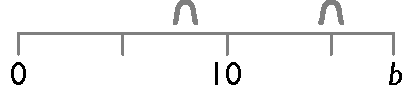
\includegraphics[width=.3\textwidth]{img/samplesetup}

Antag at pulsarens periode er~$4$, så Tycho ville tage skade på tidspunkterne $4$, $8$, $12$, osv., hvis den ikke er i ly.
Hvis Tycho forlader startpositionen (hvor den er i ly) på tidspunkt~$0$, kan den nå det første skjulested efter $8$~sekunder og blive strålingsskadet på tidspunkt~$4$ (men ikke på tidspunkt $8$, idet den er i ly).
Fortsætter den uden at stoppe, ankommer den til hjemmebasen på tidspunkt~$18$ og pådrager sig $d+d$ flere enheder af strålingsskade (på tidspunkterne $12$ og $16$, henholdsvis).
På denne måde vil den samlet pådrage sig $d+d+d=3d$ enheder af strålingsskader og $18$ enheder af miljøskader.
Hvis Tycho i stedet venter ved det $2$.~skjulested (ved position~$15$) i $1$~sekund, forårsager pulsen på tidspunkt~$16$ ingen skade, og Tycho når hjemmebasen på tidspunkt~$19$ med et samlet antal skader på $2d + 19$.
Dette er bedre for de fleste værdier af $d$.
De to situationer er vist her:

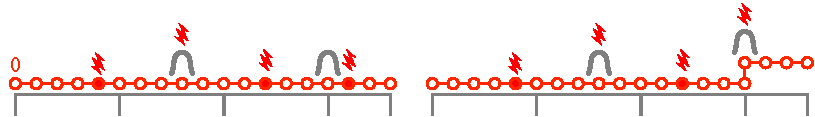
\includegraphics[width=.8\textwidth]{img/sample1_2.pdf}

Hvis pulsarens periode er $10$, kan Tycho vente ved startpositionen i $2$~sekunder og derefter bare køre hjem uden at standse ved nogen skjulesteder.
Dermed passerer han det første skjulested (på position $8$) præcis på det rigtige tidspunkt, når pulsaren blusser op, og ankommer til hjemmebasen på tidspunkt~$20$, med i alt $20$~enheder miljøskade og ingen strålingsskade overhovedet.

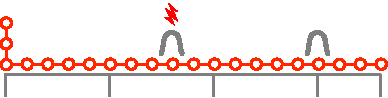
\includegraphics[width=.4\textwidth]{img/sample3.pdf}

\section*{Indlæsning}

Den første linje består af fire heltal $b$, $p$, $d$, og $n$, adskilte af enkelt mellemrum:
hjemmebasens placering~$b$,
pulsarens periode~$p$,
den ekstra strålingsskade~$d$ forårsaget af pulsaren og
antallet~$n$ af skjulesteder.
De følgende $n$ linjer indeholder hvert et heltal, der angiver skjulestedernes placeringer $a_1$, $\ldots$, $a_n$, med
$0<a_1<\cdots <a_n< b$. % constraint:shelterbounds, constraint:sortedshelters

\section*{Udskrift}

Udskriv et enkelt heltal: det mindste mængde skader, Tycho skal tage for at nå~$b$.

\section*{Begrænsninger og pointgivning}

Du kan antage, at
$1 \leq p < b$ % constraint:pulsehappens
og
$0 \leq n < b$. % constraint:sheltersfit
Der gælder altid
$1\leq b\leq 10^{12}$, % constraint:b
$0\leq d \leq 10^6$ %constraint:d
og
$0\leq n \leq 10^5$. % constraint:n

Din løsning vil blive testet på en række testgrupper, hver med en vist antal point.
Hver testgruppe indeholder en række testfald.
For at opnå point for en testgruppe skal du løse alle testfald i testgruppen.
Din endelige score vil være den højeste score for en enkelt indsendelse.

\medskip
\begin{tabular}{lll}
Gruppe & Point & Begrænsninger \\\hline
$1$ & $8$ & $p\leq 10^6$ og Tycho behøver ikke at vente \emph{efter} at have forladt position~$0$.$^*$ \\ % constraint:nowait
$2$ & $5$ & $b\leq 1000$, $p\leq 100$, $n\leq 10$ \\
$3$ & $7$ & $b\leq 1000$ \\
$4$ & $15$ & $p\leq 10^6$, $n\leq 1000$\\
$5$ & $20$ & $p\leq 100$\\
$6$ & $35$ & $p\leq 10^6$\\
$7$ & $10$ & \emph{Ingen yderligere begrænsninger}
\end{tabular}

\medskip
\noindent $^*$ I testgruppe~$1$ kan Tycho godt skulle vente ved position~$0$, \emph{inden} den begynder at køre.
Eksemplerne $2$, $3$ og $4$ tilhører testgruppe~$1$.





